\documentclass[10pt,pdf,hyperref={unicode}]{beamer}

\mode<presentation>
{
\usetheme{boxes}
\beamertemplatenavigationsymbolsempty

\setbeamertemplate{footline}[page number]
% \usecolortheme{seagull}
\setbeamersize{text margin left=0.5em, text margin right=0.5em}
}

\usepackage[utf8]{inputenc}
\usepackage[english, russian]{babel}
\usepackage{bm}
\usepackage{multirow}
\usepackage{ragged2e}
\usepackage{indentfirst}
\usepackage{multicol}
\usepackage{subfig}
\usepackage{amsmath,amssymb}
\usepackage{enumerate}
\usepackage{mathtools}
\usepackage{comment}
\usepackage{multicol}

\usepackage[all]{xy}

\usepackage{tikz}
\usetikzlibrary{positioning,arrows}

\tikzstyle{name} = [parameters]
\definecolor{name}{rgb}{0.5,0.5,0.5}

\usepackage{caption}
\captionsetup{skip=0pt,belowskip=0pt}

\newtheorem{rustheorem}{Теорема}
\newtheorem{russtatement}{Утверждение}
\newtheorem{rusdefinition}{Определение}

% colors
\definecolor{darkgreen}{rgb}{0.0, 0.2, 0.13}
\definecolor{darkcyan}{rgb}{0.0, 0.55, 0.55}

\AtBeginEnvironment{figure}{\setcounter{subfigure}{0}}% Resets subfigure counter at start of figure environment

\captionsetup[subfloat]{labelformat=empty}

%----------------------------------------------------------------------------------------------------------

\title[Пример слайдов по работе]{Пример слайдов по работе \\ курса}
\author{А.\,О.\,Фамилия}

\institute[]{Московский физико-технический институт}
% \institute[]{Конференция МФТИ}
%\date[2021]{\small Московский физико-технический институт\\04\;декабря\;2021\,г.}
%\institute[]{Конференция \\ <<Математические методы распознавания образов>>}
\date[2022]{\small 10\;февраля\;2022\,г.}

%---------------------------------------------------------------------------------------------------------
\begin{document}

\begin{frame}
\titlepage
\end{frame}

%----------------------------------------------------------------------------------------------------------
\section{Априорное распределение параметров моделей}
\begin{frame}{Априорное распределение параметров моделей}
\bigskip
Исследуется проблема выбора моделей глубокого обучения. Для выбора моделей используется связный байесовский вывод. Для снижения размерности пространства параметров при выборе модели используется информация об их априорном и апостериорном распределениях. 
\begin{block}{Цель исследования~---}
предложить метод задания априорного распределения параметров модели глубокого обучения с учетом накопленной информации о решаемой задаче.
\end{block}
\begin{block}{Требуется предложить}
\justifying
\begin{enumerate}[1)]
\item метод выбора модели, основанный на использовании привилегированной и накопленной информации,
\item метод выравнивания структур параметрических моделей,
\item метод снижения размерности пространства параметров моделей.
\end{enumerate}
\end{block}
\begin{block}{Решение}
Для назначения априорного распределения параметров при выборе моделей глубокого обучения используются апостериорные распределения параметров ранее полученных моделей.
\end{block}
\end{frame}
%---------------------------------------------------------------------------------------------------------
\section{Привилегированное обучение Вапника и Хинтона}
\begin{frame}{Привилегированное обучение {\color{red}В.\,Н.\;Вапника\footnotemark} и \\ \hfill\hfill\hfill\hfill\hfill дистилляция~{\color{blue}Дж.\;Хинтона\footnotemark}}
%\justifying
Заданы
\begin{enumerate}[1)]
    \item признаки~$\mathbf{x}_i \in \mathbb{R}^{n}$ и привилегированные признаки~$\mathbf{x}^*_i \in \mathbb{R}^{n^*}$,
    \item целевая переменная~$y_i \in \mathbb{Y}$,
    \item индексы объектов, для которых известна привилегированная информация $\mathcal{I},$ а для которых она не известна $\bar{\mathcal{I}}$.
\end{enumerate}

Модели учителя~$\mathbf{f}:\mathbb{R}^{n^*} \to \mathbb{Y}^\prime$ и ученика~$\mathbf{g}:\mathbb{R}^{n} \to \mathbb{Y}^\prime$~--- пространство оценок.

Ответы $\mathbf{s}_i = \mathbf{f}\bigr(\mathbf{x}_i^*\bigr)$ функции $\mathbf{f}$ для объектов~$\mathbf{x}^*_i$.

\bigskip

Требуется выбрать модель ученика~$\mathbf{g}$ из множества
\[
	\mathfrak{G} = \left\{\mathbf{g}| \mathbf{g}:\mathbb{R}^{n} \to \mathbb{Y}^\prime\right\}.
\]
Оптимизационная задача:
\[
	\mathbf{g} = \arg\min_{\mathbf{g} \in \mathfrak{G}} \mathcal{L}\bigr(\mathbf{g}, \mathbf{f}, \mathbf{X}, \mathbf{X}^{*}, \mathbf{y},\mathbf{s}\bigr),
\]
где $\mathcal{L}$~--- функция ошибки.

\bigskip
\footnotetext[1]{\textit{Lopez-Paz D., Bottou L., Scholkopf B., Vapnik V.} {\color{red}Unifying distillation and privileged information} // ICLR, 2016.}
\footnotetext[2]{\textit{Hinton G., Vinyals O., Dean J.} {\color{blue}Distilling the knowledge in a neural network} // NIPS, 2015.}
\end{frame}

%---------------------------------------------------------------------------------------------------------
\section{ФРЕЙМЫ}
\begin{frame}
\frametitle<1>{Задача оптимизации параметров модели}
\frametitle<2>{Байесовский выбор модели}
\frametitle<3>{Байесовская дистилляция модели}

\begin{minipage}[t][4.1cm][t]{\textwidth}
~\\[-2mm]
\begin{equation*}
\xymatrix{
% First Line
\parbox{3em}{
\footnotesize Задача \\ оптимизации
}
&
\parbox{3em}{
\centering
$\hat{\mathbf{w}}, \hat{\mathbf{A}}_{w}\ar[r]^{g}$
}
& 
\hat{y}\ar[rr]
&
\parbox{3em}{
\centering
}
& 
\parbox{10em}{
\centering
$
\only<1>{\mathcal{L}\bigr(\hat{\mathbf{w}},\hat{\mathbf{A}}_{\text{w}}|y, \hat{y}\bigr)}
\only<2>{\mathcal{L}\bigr(\hat{\mathbf{w}},\hat{\mathbf{A}}_{\text{w}}|y, \hat{y}, {\color{blue}\mathbf{w}_0, \mathbf{A}_0}\bigr)}
\only<3>{\mathcal{L}\bigr(\hat{\mathbf{w}},\hat{\mathbf{A}}_{\text{w}}|{\color{blue} s, }y, \hat{y}, {\color{blue}\mathbf{w}_0, \mathbf{A}_0}\bigr)}
\ar@/_2pc/[lll]
$
}
\\
% Second Line
\only<2-3>{
\parbox{3em}{\footnotesize Дополнительная \\ информация}
}
&
\only<2>{\color{blue} \mathfrak{G} \ar[u]}
\only<3>{\mathfrak{G} \ar[u]}
&
\only<3>{\color{blue} s \ar[urr]}
&
\only<3>{\color{blue} \hat{\mathbf{u}}, \hat{\mathbf{A}}_{\text{u}} \ar[r] \ar[l]^{f}}
&
\only<2-3>{\color{blue} \left(\mathbf{w}_0, \mathbf{A}_0\right) \ar[u]}
\\
% Third Line
\parbox{3em}{\footnotesize Выборка}
&
&
\parbox{3em}{
\centering
$
\only<3>{\color{blue} (\mathbf{x}^{*}, y) \ar[u]}
$
}
& 
\only<1-2>{\left(\mathbf{x}, y\right) \ar[uul] \ar[uur]}
\only<3>{\left(\mathbf{x}, y\right) \ar@{.>}[uul] \ar@{.>}[uur]}
&
}
\end{equation*}
\end{minipage}

\vfill
\vspace{0.5cm}
\begin{itemize}
%\setlength\itemsep{0.1em}
\item[] Выборка
    \only<1-2>{
        $\mathfrak{D}\ni(\mathbf{x},y)$,
        %\left\{\mathbf{x}_i, y_i\right\}_{i=1}^{m},\quad 
	    $\mathbf{x}\in\mathbb{R}^{n}, y\in\mathbb{Y}$
	    % где~$m$~число объектов, $n$~число признаков.
    }
    \only<3>{
        $\mathfrak{D}\ni(\mathbf{x},{\color{blue}\mathbf{x}^{*}},y)$,
        %\left\{(\mathbf{x}_i, {\color{blue}\mathbf{x}_i^{*}}, y_i)\right\}_{i=1}^{m},
        $\quad \mathbf{x} \in \mathbb{R}^{n}, y \in \mathbb{Y}, \quad \text{дополнительно~} {\color{blue} \mathbf{x}^*\in \mathbb{R}^{n^{*}}}$ 
        %где~$m$~число объектов, $n$~число признаков, {\color{blue}$n^*$}~число признаков
    }
    \item[] Модели $\mathfrak{G}\ni\mathbf{g}: \mathbb{R}^{n}\times\mathbb{R}^{n_{w}} \to \mathbb{Y}^\prime$
        \only<1-2>{}
        \only<3>{
            $\quad\text{и учитель~}{\color{blue}\mathbf{f}:\mathbb{R}^{n^{*}}\times \mathbb{R}^{n_{w}^{*}} \to \mathbb{Y}^\prime}$
        }
    \item[] Прогноз $\hat{y} = g\bigr(\mathbf{x}, \hat{\mathbf{w}})$
        \only<1>{}
        \only<2>{}
        \only<3>{
            $\quad \text{и~}
            {\color{blue} s = f\bigr(\mathbf{x}^{*}, \hat{\mathbf{u}})}$}
    \item[]<2-3> Априорное распределение 
        \only<2>{
            \color{blue}$\mathbf{w} \sim \mathcal{N}\bigr(\mathbf{w}_0, \mathbf{A}_0\bigr)$}
        \only<3>{
            $\mathbf{w} \sim \mathcal{N}\bigr({\color{blue}\mathbf{w}_0\bigr(\hat{\mathbf{u}}, \hat{\mathbf{A}}_{\text{u}}\bigr)}, {\color{blue}\mathbf{A}_0\bigr(\hat{\mathbf{u}}, \hat{\mathbf{A}}_{\text{u}}\bigr)}\bigr)$.
        }
    %\item[] Функция потерь
    %    \only<1>{
    %        $\mathcal{L}\bigr(\hat{\mathbf{w}},\hat{\mathbf{A}}_{\text{w}}|y, %\hat{y}\bigr)$.}
    %    \only<2>{
    %        $\mathcal{L}\bigr(\hat{\mathbf{w}},\hat{\mathbf{A}}_{\text{w}}|y, %\hat{y}, {\color{blue}\mathbf{w}_0, \mathbf{A}_0}\bigr)$.}
    %    \only<3>{
    %        $\mathcal{L}\bigr(\hat{\mathbf{w}},\hat{\mathbf{A}}_{\text{w}}|{\color{bl%ue} s, }y, \hat{y}, {\color{blue}\mathbf{w}_0, \mathbf{A}_0}\bigr)$.}
    \item[] Оптимизационная задача
        \only<1-2>{
            \[
            \hat{\mathbf{w}}, \hat{\mathbf{A}}_{w} = \mathop{\arg\min}_{\mathbf{w} \in \mathbb{R}^{n_{w}}, \mathbf{A} \in \mathbb{R}^{n_{w}\times n_{w}}} \mathcal{L}\bigr(\mathbf{w},\mathbf{A}_{\text{w}}|\mathfrak{D},\mathbf{g}\bigr)
            \]}
        \only<3>{
            \[
            \hat{\mathbf{w}}, \hat{\mathbf{A}}_{w} = \mathop{\arg\min}_{\mathbf{w} \in \mathbb{R}^{n_{w}}, \mathbf{A} \in \mathbb{R}^{n_{w}\times n_{w}}} \mathcal{L}\bigr(\hat{\mathbf{w}},\hat{\mathbf{A}}_{\text{w}}|{\color{blue} \mathbf{s}}, \mathfrak{D}, {\color{blue}\mathbf{w}_0, \mathbf{A}_0}, \mathbf{g},{\color{blue}\mathbf{f}}\bigr)
            \]}
\end{itemize}
\end{frame}

%----------------------------------------------------------------------------------------------------------
\section{Оптимизация модели ученика на основе учителя~и привилегированных признаков}
\begin{frame}{Оптимизация модели ученика на основе учителя~и привилегированных признаков}
~\\[-1mm]
Заданы
\begin{enumerate}[1)]
	\item $\mathbf{x}^*_i = \mathbf{x}_i$, {\color{red} $\mathbf{x}^*_i \not= \mathbf{x}_i$} для всех $i \in \{1, 2, \cdots, m\}$,
	\item $y_i \in \mathbb{Y}=\{1, \cdots, K\}, \quad \mathbb{Y}^\prime=\mathbb{R}^{K}$.
\end{enumerate}

\medskip
Параметрические семейства учителя и ученика:
\[
\setlength\abovedisplayskip{0pt}
\mathfrak{F}^{\color{red}*}_{\text{cl}} = \left\{\mathbf{f}| \mathbf{f} = \text{softmax}\bigr(\mathbf{v}^{\color{red}*}\bigr(\mathbf{x}^{\color{red}*}\bigr)/T\bigr), \quad \mathbf{v}^{\color{red}*}: \mathbb{R}^{n^{\color{red}*}} \to \mathbb{R}^K \right\},
%\setlength\belowdisplayskip{0pt}
\]
\[
%\setlength\abovedisplayskip{0pt}
\mathfrak{G}_{\text{cl}} = \left\{\mathbf{g}| \mathbf{g} = \text{softmax}\bigr(\mathbf{z}\bigr(\mathbf{x}\bigr)/T\bigr), \quad \mathbf{z}: \mathbb{R}^n \to \mathbb{R}^K \right\},
%\setlength\belowdisplayskip{0pt}
\]
где~$\mathbf{z},\mathbf{v}^{\color{red}*}$~--- дифференцируемые по параметрам функции заданной структуры, $T$~--- параметр температуры.

\medskip
Функция ошибки
\[
\setlength\abovedisplayskip{0pt}
\begin{aligned}
   \mathcal{L}\bigr(\mathbf{g}\bigr) = &-\sum_{i=1}^{m}\underbrace{{\sum_{k=1}^{K}y^k_i\log\mathbf{g}\bigr(\mathbf{x}_i\bigr)\bigr|_{T=1}}}_{\text{исходная функция потерь}}- \sum_{i=1}^{m}\underbrace{{\sum_{k=1}^{K}\mathbf{f}\bigr(\mathbf{x}^{\color{red}*}_i\bigr)\bigr|_{T=T_0}\log\mathbf{g}\bigr(\mathbf{x}_i\bigr)\bigr|_{T=T_0}}}_{\text{слагаемое дистилляции}},
\end{aligned}
\setlength\belowdisplayskip{0pt}
\]
где~$\cdot\bigr|_{T=t}$ фиксирует температуру~$T$.

%Оптимальная модель~$\mathbf{g}$ выбирается из класса~$\mathfrak{G}_{\text{cl}}$,
Оптимальная модель выбирается из класса,
%\[\setlength\abovedisplayskip{0pt}
$\hat{\mathbf{g}} = \arg\min\limits_{\mathbf{g} \in \mathfrak{G}_{\text{cl}}} \mathcal{L}\bigr(\mathbf{g}\bigr).$
%\setlength\belowdisplayskip{0pt}\]
\end{frame}

%----------------------------------------------------------------------------------------------------------
\begin{frame}{Анализ правдоподобия выборки, выравнивание моделей с разным числом скрытых слоев}
\justifying
Вид суперпозиции модели учителя:
$$
\setlength\abovedisplayskip{0pt}
f\bigr(\mathbf{x}\bigr) = \bm{\sigma} \circ \mathbf{U}_3\circ \bm{\sigma} \circ \mathbf{U}_2\circ\bm{\sigma}\circ \mathbf{U}_1\mathbf{x},
\setlength\belowdisplayskip{0pt}
$$
Вид суперпозиции модели ученика:
$$
\setlength\abovedisplayskip{0pt}
g = \bm{\sigma} \circ \mathbf{W}_2 \circ \bm{\sigma} \circ \mathbf{W}_1, \quad \mathbf{W}_{1} \in \mathbb{R}^{1 \times 50}, \mathbf{W}_{2} \in \mathbb{R}^{50 \times 10}.
\setlength\belowdisplayskip{0pt}
$$
\begin{table}[]
\begin{center}
\resizebox{0.9\textwidth}{!}{
\begin{tabular}{|l|c|c|c|c|}\cline{1-5}
                  & Учитель           & Ученик        & Дистил.-ученик & Дистил.-ученик-все \\ \cline{1-5}
Структура            & $[10,100,50,1]$   & $[10,50,1]$       & $[10,50,1]$      & $[10,50,1]$ \\ \cline{1-5}
Число параметров    &   6050                       &       550                   &          550               &     550 \\ \cline{1-5}
Разность площадей    &  -                          &  0                      &  $\mathbf{23310}$             & $\mathbf{25506}$ \\ \cline{1-5}
\end{tabular}
}
\end{center}
\end{table}

Анализ решения задачи: интегральная разность~$\ln p\bigr(\mathbf{y}|\mathbf{X}, \mathbf{w}\bigr)$ по итерациям.
\begin{figure}[h!]
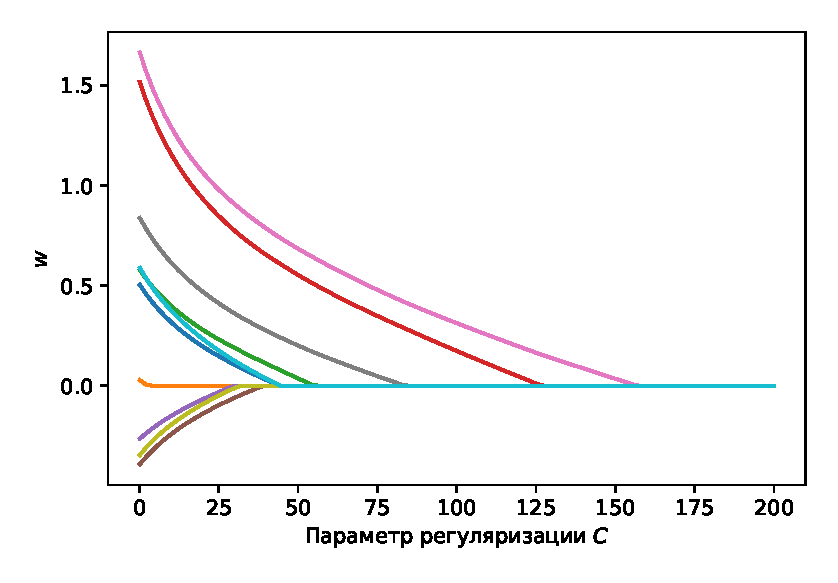
\includegraphics[width=0.4\textwidth]{../figures/log_reg_cs_exp.eps}
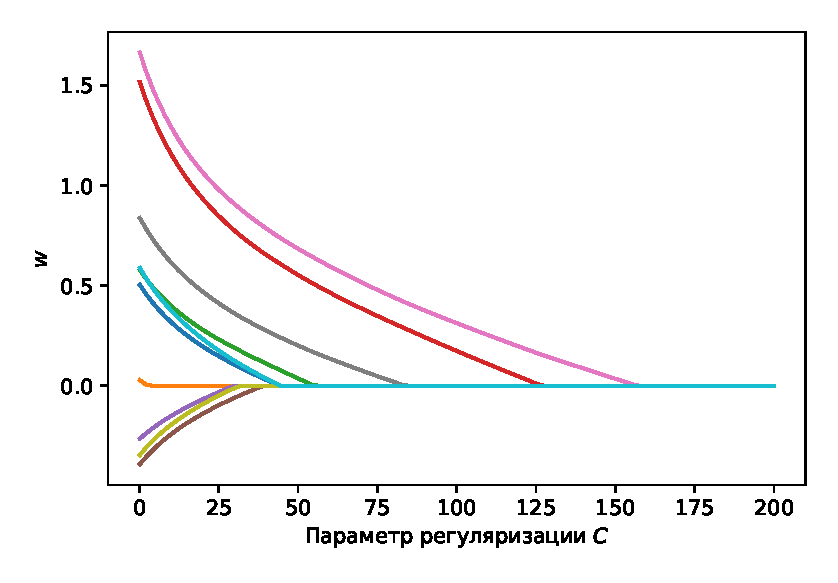
\includegraphics[width=0.4\textwidth]{../figures/log_reg_cs_exp.eps}
\end{figure}

Правдоподобие модели ученика с дистилляцией растет быстрее чем без нее.

\end{frame}

%----------------------------------------------------------------------------------------------------------
\section{Выносится на защиту}
\begin{frame}{Выносится на защиту}
\justifying
	\begin{enumerate}
	\justifying
	    \item Предложен байесовский метод выбора моделей с использованием модели учителя с привилегированной и накопленной информации.
        \item Доказаны теоремы о свойствах дистилляции, 
        \begin{itemize}
            \item[---] \emph{теоремы об эквивалентности} для дистилляции моделей в случае задачи регрессии и классификации,
            \item[---] \emph{теоремы о виде априорного распределения} параметров модели ученика в байесовской дистилляции.
        \end{itemize}
        \item Предложен метод выравнивания структур параметрических моделей. Предложен метод выбора априорного распределения параметров модели ученика с использованием апостериорного распределения параметров модели учителя для случаев
        \begin{itemize}
            \item[---] различных размерностей пространств параметров отдельных слоев,
            \item[---] различного в числа слоев нескольких моделей.
        \end{itemize}
        \item Предложены методы задания порядка на множестве параметров моделей
        \begin{itemize}
            \item[---] на основе корреляции параметров,
            \item[---] на основе оценки скорости сходимости параметров.
        \end{itemize}
        \item Предложена вероятностная интерпретации дистилляции моделей глубокого обучения. Исследованы свойства дистилляции моделей глубокого обучения.
	\end{enumerate}
\end{frame}
%----------------------------------------------------------------------------------------------------------

\end{document} 